\documentclass[11pt, a4paper, spanish, openright, twoside]{book}
\usepackage[spanish, activeacute]{babel}
\usepackage[utf8]{inputenc}
%\usepackage[top=2.5cm, bottom=2.5cm, outer=1.75cm, inner=1.75cm, heightrounded, marginparwidth=2.5cm, marginparsep=0.3cm]{geometry}	%márgenes empequeñecidos
\usepackage[top=2.95cm, bottom=2.25cm, outer=2.75cm, inner=2.75cm, heightrounded, marginparwidth=2.5cm, marginparsep=0.3cm]{geometry}	%márgenes originalmente
\usepackage{dpg}
\usepackage{fli}

\usepackage{pgf}
\usepackage{tikz}

\usepgflibrary{shapes.geometric} % LATEX and plain TEX and pure pgf
\usetikzlibrary{arrows,automata,positioning}
\tikzstyle{accepting by double}= [double distance=1.6pt,double,outer sep=.5\pgflinewidth+.8pt] % esto es algo estético.
\renewcommand\shorthandsspanish{}  % para compatibilizar spanish con tikz

%%%%%%		Figuras		%%%%%%%%%%%%%%%%%%%
\usepackage[vflt]{floatflt}		%Entorno float-figure

%%%%%%		Page style		%%%%%%%%%%%%%%%%%%%
\renewcommand{\thepage}{\arabic{page}}% Arabic page numbers\fancyhead{}
\pagestyle{fancy}
\fancyfoot{}
\fancyhead[LO,RE]{Práctica 3}	%encabezado de pares: nombre de la sección
\fancyfoot[LE,RO]{\thepage}	%abajo a izqda en pares, derecha en impares: numero de pagina
%\fancyhead[LE]{\nouppercase{\leftmark}} %cuadro izquierdo de pagina par: parte y contador
\fancyfoot[CE]{Inteligencia Artificial} 
\fancyfoot[CO]{Doble Grado Informática-Matemáticas - Universidad Complutense}
\renewcommand{\footrulewidth}{0.4pt}
\renewcommand{\headrulewidth}{0.4pt}		% linea por debajo del encabezado
\renewcommand{\sectionmark}[1]{\markright{\textbf{\thesection. #1}}}	%negrita
\renewcommand{\labelitemi}{$\circ$} %Primer itemize con circunferencia vacia
\renewcommand{\labelitemii}{$\cdot$} %Segundo itemize con punto pequeño \cdot
\renewcommand*{\thesection}{\arabic{section}}	% Hace que no apareca el indice de capitulos y que comience en section

%%%%%%		Others		%%%%%%%%%%%%%%%%%%%
\setlength{\leftmarginii}{0em} %Segundo itemize sin sangria
\setlength{\leftmarginiii}{1em} %Tercer itemize casi sin sangria
\renewcommand{\labelitemiii}{ }
\pagenumbering{roman}
\addto{\captionsspanish}{\renewcommand*{\contentsname}{Índice}} %Cambia "Indice general" por "Indice"



\begin{document} 
\title{\Huge{\textsc{Inteligencia Artificial}} \\
	\vspace{0.7cm}
	 \textsc{\Large{Práctica 3}} \\
	\vspace{1.5cm}
	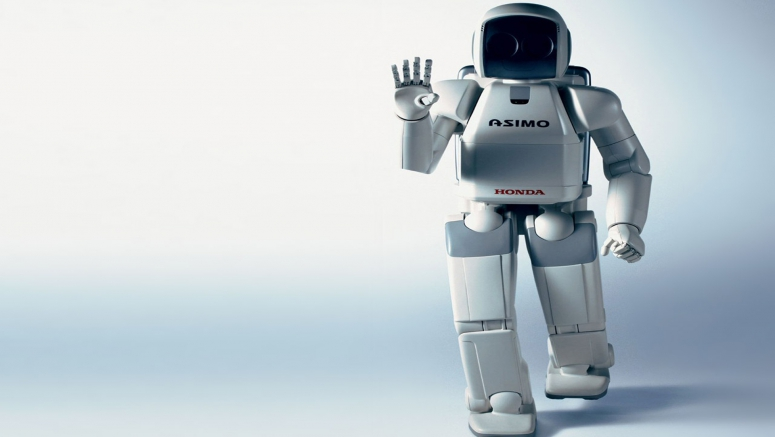
\includegraphics[scale=0.45]{robotHonda}}
\author{\textsc{Grupo 3:}\\
	Enrique Ballesteros Horcajo\\
	Ignacio Iker Prado Rujas}
\date{\Today}
\maketitle

\newpage
\mbox{}
\thispagestyle{empty}						% Hoja en blanco, sin numeros ni nada
\newpage


\tableofcontents 							%INDICE hipervinculado

\newpage
\mbox{}
\thispagestyle{empty}						% Hoja en blanco, sin numeros ni nada
\newpage

\pagenumbering{arabic}						% Pone el contador de paginas a 1 y ahora en numeros normales

\vspace{3cm}


\newpage



\begin{section}{Introducción: Jarras Demo}

	\textbf{Problema:} \textit{Se tienen dos jarras vacías con capacidades de 3 y 4 litros respectivamente pero sin ninguna marca de medida parcial. Las jarras pueden vaciarse o llenarse de agua, así como verter el contenido de una a otra. El objetivo consiste en tener exactamente 2 litros de agua en la jarra de 4 litros.}

	Vamos a poder realizar tres tipos de operaciones con las jarras:
	
	\begin{itemize}

		\item Vaciar jarra totalmente. Deja la jarra sin agua.
		\item Llenar jarra totalmente. Deja la jarra al máximo de su capacidad.
		\item Verter una jarra en la otra. Echa agua de una jarra en la otra hasta que la origen se llena 
			o la destino se llena. No se derrama ninguna gota en el proceso.
	\end{itemize}
	El estado va a ser una dupla, cantidad de agua en la jarra de 4 litros y cantidad de agua en la jarra de 3 (en ese orden):
	\begin{itemize} 
		
		\item Estado $= (X, Y)$, i.e., la jarra de 4 litros tiene $X(\le 4)$ litros y la jarra de 3 litros tiene $Y(\le 3)$ litros.
		\item Estado inicial $= (0, 0)$, i.e., ambas jarras comienzan vacías.
		\item Estado objetivo $= (2, Y)$, ya que no nos importa cuanto quede en la jarra de 3 litros.
		
	\end{itemize}
	
	Las operaciones serán, incluyendo precondiciones y postcondiciones:
		\begin{itemize}
		\item \texttt{LL4} $\rightarrow$ Llenar la jarra de 4.
			\begin{itemize}
			\item \underline{Precondiciones}: $ (X, Y)$ : $X < 4$.
			\item \underline{Postcondición}: $(4, Y)$.
			\end{itemize}
		
		\item \texttt{VA4} $\rightarrow$ Vaciar la jarra de 4.
			\begin{itemize}
			\item \underline{Precondiciones}: $(X, Y)$ : $X > 0$.
			\item \underline{Postcondición}: $(0, Y)$.
			\end{itemize}

		\item \texttt{VE4} $\rightarrow$ Verter la jarra de 4 en la de 3.
			\begin{itemize}
				\item \underline{Precondiciones}: $(X, Y)$ : $X > 0, Y < 3$.
				\item \underline{Postcondiciones}: $(X', Y')$ : 
				\begin{itemize}
					\item Cabe toda la jarra cuatro:  $(X + Y) \le 3$ ; Final: $X'= 0$, $Y' = X + Y$.
					\item No cabe entera: $(X + Y) > 3$ ;	Final: $X'= X - (3 - Y)$, $Y'= 3$.
				\end{itemize}
			\end{itemize}

		\item \texttt{LL3} $\rightarrow$ Llenar la jarra de 3.
			\begin{itemize}
			\item \underline{Precondiciones}: $(X, Y)$ : $Y < 3$.
			\item \underline{Postcondición}: $(X, 3)$.
			\end{itemize}
		
		\item \texttt{VA3} $\rightarrow$ Vaciar la jarra de 3.
			\begin{itemize}
			\item \underline{Precondiciones}: $(X, Y)$ : $Y > 0$.
			\item \underline{Postcondición}: $(X, 0)$.
			\end{itemize}
		\item \texttt{VE3} $\rightarrow$ Verter la jarra de 3 en la de 4.
			\begin{itemize}
				\item \underline{Precondiciones}: $(X, Y)$ : $X < 4$, $Y > 0$.
				\item \underline{Postcondiciones}: $(X', Y')$ : 
				\begin{itemize}
					\item Cabe toda la jarra tres: $(X + Y) \le 4$.  Final: $X'= X + Y$, $Y' = 0$.
					\item No cabe entera: $(X + Y) > 4$. Final: $X'= 4$, $Y'= Y - (4 - X)$.
				\end{itemize}
			\end{itemize}
		\end{itemize}
	
	Cada operación que se realiza cuesta 1, luego el coste de una 
				solución es el número de operaciones hasta que llegas a ella.
		

		
\end{section}

\begin{section}{Búsqueda en anchura}
	
\texttt{
	JarrasBFSDemo(Anchura)--> \\
	Action[name==Llenar jarra 3]		\\
	Action[name==Verter jarra 3] 		\\ 
	Action[name==Llenar jarra 3]		\\
	Action[name==Verter jarra 3]		\\
	Action[name==Vaciar jarra 4]		\\
	Action[name==Verter jarra 3]		\\
	pathCost : 6.0					\\
	nodesExpanded : 11			\\
	queueSize : 1					\\
	maxQueueSize : 3				
}

La búsqueda en anchura o por niveles, explora nivel a nivel siguiendo el orden de instrucciones dado en \texttt{JarrasActionsFunction}, por ello encuentra la solución que 
empieza por llenar jarra 3 y no por llenar jarra 4, pues ese movimiento está antes en el \texttt{Set$<$Action$>$}. Además, al ser el coste proporcional a la profundidad, encontramos una solución óptima.
 Si hubiese alguna solución a menor profundidad la habría encontrado.

\end{section}

\begin{section}{Búsqueda en profundidad}

\texttt{
	JarrasDLSDemo(Profundidad limitada(9))-->	\\
	Action[name==Llenar jarra 3]		\\
	Action[name==Vaciar jarra 3]		\\
	Action[name==Llenar jarra 3]		\\
	Action[name==Verter jarra 3]		\\
	Action[name==Llenar jarra 3]		\\
	Action[name==Verter jarra 3]		\\
	Action[name==Vaciar jarra 4]		\\
	Action[name==Verter jarra 3]		\\
	pathCost : 8.0					\\
	nodesExpanded : 107			\\
}

\texttt{
	JarrasDFSDemo(Profundidad)-->	\\
	Action[name==Llenar jarra 4]		\\
	Action[name==Verter jarra 4]		\\
	Action[name==Vaciar jarra 3]		\\
	Action[name==Verter jarra 4]		\\
	Action[name==Llenar jarra 4]		\\
	Action[name==Verter jarra 4]		\\
	pathCost : 6.0					\\
	nodesExpanded : 6				\\
	queueSize : 2					\\
	maxQueueSize : 3				
}

\end{section}

\begin{section}{Búsqueda $A^*$ con heurística \textit{Kiker}}

\texttt{
	JarrasAStarDemo(Kiker heuristic)-->	\\
	Action[name==Llenar jarra 4]		\\
	Action[name==Verter jarra 4]		\\
	Action[name==Vaciar jarra 3]		\\
	Action[name==Verter jarra 4]		\\
	Action[name==Llenar jarra 4]		\\
	Action[name==Verter jarra 4]		\\
	pathCost : 6.0					\\
	nodesExpanded : 11			\\
	queueSize : 1					\\
	maxQueueSize : 3				
}

La heurística  \textit{Kiker} no aporta nada respecto de, por ejemplo, la búsqueda en anchura ya que es una heurística bastante mala. Concretamente no es 
una heurística admisible, ya que estando a un nivel de la solución nos da un 2, y estando a tres niveles nos da un 1. Como no es admisible tampoco es consistente.


\end{section}
\begin{section}{Búsqueda $A^*$ con heurística \textit{Jarras}}

\texttt{
	JarrasAStarDemo2(Jarras heuristic)-->	\\
	Action[name==Llenar jarra 4]		\\
	Action[name==Verter jarra 4]		\\
	Action[name==Vaciar jarra 3]		\\
	Action[name==Verter jarra 4]		\\
	Action[name==Llenar jarra 4]		\\
	Action[name==Verter jarra 4]		\\
	pathCost : 6.0					\\
	nodesExpanded : 12			\\
	queueSize : 1					\\
	maxQueueSize : 3				
}

\end{section}
\begin{section}{Notas}
	Una heurística (informática) es \textbf{admisible} si nunca sobreestima el costo de alcanzar el objetivo, o sea, 
que en el punto actual la estimación del costo de alcanzar el objetivo nunca es mayor que el menor costo posible.

	Una heurística $h(n)$ es \textbf{consistente} si, para todo nodo $n$ y todo sucesor $n'$ de $n$ generado por cualquier acción $A$, el costo estimado de alcanzar el objetivo desde $n$ no es mayor que el costo de obtener $n'$ más el costo estimado de obtener el objetivo desde $n'$.

	Una heurística $h'(n)$ es consistente si, para cada nodo $n$ y cada sucesor $n'$ de $n$, el coste 
	estimado de alcanzar el objetivo desde $n$ no es mayor que el coste real de 
	alcanzar $n'$ más el coste estimado de alcanzar el objetivo desde $n'$.
		\begin{itemize}
		\item  $h'(n) <= c(n, n') + h'(n')$ (desigualdad triangular).
		\item  $h'$  ha de ser localmente consistente con el coste de los arcos.
		\item Toda heurística consistente también es admisible (pero no al revés).
		\item Si $h'$ es consistente entonces los valores de $f'$ a lo largo de cualquier 
		camino no disminuyen ($f'$ monótona no decreciente).
		\end{itemize}

$$\boxed{h(n) \le c(n, A, n') + h(n')}$$
\end{section}

\begin{section}{Conclusiones}
	
	
	
\end{section}

\begin{thebibliography}{9}

\bibitem{aima}
	Russell, S.; Norvig, P, \\
	\emph{Artificial Intelligence, a modern aproach}.\\
	New Jersey: Pearson, 2010.
	
\bibitem{clase}
	Apuntes y transparencias de Inteligencia Artificial, \\
	Doble Grado Matemáticas - Ing. Informática, U.C.M., 2014-2015.

\end{thebibliography}


\end{document}

